%-----------------------------------------------------------------------------
% Title, Author, Date
%-----------------------------------------------------------------------------

\title{A spatial logit model for Bayesian hierarchical semiparametric regression}
\author{
        Spencer Woody\footnote{The University of Texas at Austin, Department of Statistics and Data Science. Data and \textsf{R} script used for this analysis available at \texttt{github.com/spencerwoody/NOLA} } \\
				\texttt{spencer.woody@utexas.edu}
}
\date{\today}

%-----------------------------------------------------------------------------
% Document Class
%-----------------------------------------------------------------------------

\documentclass[11pt]{article}
\usepackage{cite}


%-----------------------------------------------------------------------------
% Packages
%-----------------------------------------------------------------------------

\usepackage{graphicx}
\usepackage{amsmath} 
\usepackage{amssymb}
\usepackage{listings}
\usepackage{enumerate} 


% Theorems, corollaries, lemma
\usepackage{amsthm}
\usepackage[utf8]{inputenc}
\usepackage[english]{babel}
\newtheorem{theorem}{Theorem}[section]
\newtheorem{corollary}{Corollary}[theorem]
\newtheorem{lemma}[theorem]{Lemma}

% Appendix
% \usepackage[toc,page]{appendix}

% Fonts
\usepackage{mathpazo}
\usepackage{avant}
\usepackage{inconsolata}

% Margins
\usepackage[margin=1in]{geometry}

% Define new commands
\usepackage{bm,upgreek}

\newcommand{\tr}{\text{tr}}
\newcommand{\pN}{\mathcal{N}}
\newcommand{\I}{\mathcal{I}}
\newcommand{\R}{\textsf{R} }
\newcommand{\1}{\mathbf{1}}
\newcommand{\0}{\mathbf{0}}
\newcommand{\x}{\mathbf{x}}
\newcommand{\tee}{\mathbf{t}}
\newcommand{\f}{\mathbf{f}}
\newcommand{\K}{\mathbf{K}}
\newcommand{\g}{\mathbf{g}}
\newcommand{\h}{\mathbf{h}}
\newcommand{\y}{\mathbf{y}}
\newcommand{\YY}{\mathbf{Y}}
\newcommand{\bmpsi}{\bm{\uppsi}}

%-----------------------------------------------------------------------------
% Begin Document -----
%-----------------------------------------------------------------------------


\begin{document}
\maketitle


%-----------------------------------------------------------------------------
%-----------------------------------------------------------------------------
%-----------------------------------------------------------------------------
%---------------------------    START OF TEXT    -----------------------------
%-----------------------------------------------------------------------------
%-----------------------------------------------------------------------------
%-----------------------------------------------------------------------------






%-----------------------------------------------------------------------------
% ABSTRACT
%-----------------------------------------------------------------------------

\begin{abstract}
RNA-seq has emerged as the predominant technology for gene expression analysis. Modeling approaches must take into account the fact that there data are in the form of overdispersed counts. Existing models use the negative binomial distribution. However, there are few existing analysis pipelines which can infer a continuous time course of gene expression. In this paper we present a negative binomial regression model with a logit link on an underlying latent nonparametric time course function taken from a hierarchical Gaussian process to model dynamic gene expression. The advantages of this approach are that it can pool information across replicates and handle the case of samples collected at irregular time intervals. We also present a Gibbs sampler for implementing the model. The model is applied to an RNA-seq time series dataset from an experiment tracking the cellular response of \emph{E. coli} to starvation conditions. We conclude by listing potential extensions of the model and other future work to be done. This paper is written as a final project for the spring 2017 semester course SDS 383D course taught by Professor James Scott at UT-Austin.
\end{abstract}









%-----------------------------------------------------------------------------
% INTRODUCTION
%-----------------------------------------------------------------------------

\section{Introduction}
Recently there has been a proliferation of next-generation sequencing technologies used in bioinformatics. RNA-seq has become the new dominant tool for gene expression analysis, which may be used to infer gene regulatory networks and measure cellular response to external stimuli, to name just a few examples.  \cite{PG} \cite{NBregression}

As opposed to microarray data, where gene expression is measured as a continuous variable, RNA-seq data are in the form of counts and are thus discrete. Furthermore, RNA-seq data are often overdispersed (i.e., the variance is larger than the mean), so the Poisson distribution, which has equal variance and mean, is inappropriate to use. Popular analysis pipelines, such as DESeq2 {DESeq2} and edgeR {edgeR}, use the negative binomial distribution. These techniques often fit a generalized linear model (GLM) with some sort of link function, such as the logarithmic link. This may be well suited for tasks such as differential expression between several conditions (e.g. experiment and control), but they are not adept at modeling the continuous time course of gene expression which is likely nonlinear.

In response I propose a negative binomial regression model with a logit link on a latent hierarchical Gaussian process. The motivation for this model comes from {GPmicroarray}, where the authors use a hierarchical Gaussian process to model time series microarray data for samples with multiple replicates. Their approach accounts for hierarchy at the replicate level, but may also be extended to cases like data fusion where an experimenter would also like to pool information across related groups. In our case, we account for the discrete nature of RNA-seq data with the linked negative binomial regression. This allows us to use the same Gaussian process framework in a discrete data context, and the same extensions mentioned in {GPmicroarray} like clustering and data fusion should be applicable to this case too.

% \paragraph{Outline}
% The remainder of this article is organized as follows.
% Section~{Model} gives account of previous work.
% Our new and exciting results are described in Section~{Inference}, Section~{Experiment}, Section~{Conclusion}.
% Finally, Appendix~{mainlemma} gives the conclusions.









%-----------------------------------------------------------------------------
% THE MODEL
%-----------------------------------------------------------------------------

\section{Model}\label{Model}

We model the probability of reopening store $j$ along street $i$ as $\Pr(y_{ij} = 1) = 1/\{ 1 + \exp(-\psi_{ij}) \}$, using a probit link on a latent value $\psi_{ij}$ which comes from 
%
%
%
\begin{align*}
	\psi_{ij} &= x_{ij}^T\beta + f_i(\mathbf{s}_{ij}),
\end{align*}
%
%
where $\mathbf{s}_{ij}$ is the geographic location ,
%
%
%
\begin{align*}
	\bmpsi_{i} &= X_i\beta + \f_i, \\
	\f_i &= \left\{ f(\mathbf{s}) \sim \text{GP}(0, k_f(\mathbf{s},\mathbf{s}')) : \mathbf{s} \in \mathcal{S}_i \right\}
\end{align*}
%
%
%
for some covariance function $k_f$ which depends on vector hyperparameters $\bm{\uptheta}$. The vector $\f_i$ can be seen as coming from 
%
%
\begin{align*}
	(\f_i | \bm{\uptheta}) &\sim \pN(\mathbf{0}, \K_{i}),
\end{align*}
%
%
%
where $\K_{i}$ is the matrix such that its $(j, j')$ element is $k_f(\mathbf{s}_{ij}, \mathbf{s}_{ij'})$. Then we can see that
%
%
%
\begin{align*}
	(\bmpsi_i | \f_i, \bm{\uptheta}) &\sim \pN(X_i\beta, \K_i).
\end{align*}
%
%
%
The model specification is complete when we assign a noninformative flat prior for $\beta,$ 
%
%
\begin{align*}
	\pi(\beta) &\propto 1
\end{align*} 




\subsection{Covariance Function}

A good covariance function is the $\text{Mat\'{e}rn(5/2)},$
%
%
%
\begin{align*}
	k_f(\mathbf{s},\mathbf{s}') &= \tau^2 \exp\left\{ 1 + \sqrt{5} \cdot \frac{d}{b} + \frac{5}{3} \cdot \frac{d^2}{b^2} \right\} \exp \left\{ -\sqrt{5} \cdot \frac{d}{b} \right \} , \; d = \| \mathbf{s} - \mathbf{s}' \|, 
\end{align*}
%
%
with hyperparamters $\bm{\uptheta} = (\tau^2, b)$, and $d$ is calculated as some measure of distance between $\mathbf{s}$ and $\mathbf{s}'.$ Since the data here are geographic coordinates, we use the distance calculated from the Haversine formula. 


%-----------------------------------------------------------------------------
% INFERENCE
%-----------------------------------------------------------------------------

\section{Inference}\label{Inference}

Build an MCMC algorithm :)

\subsection{Data augmentation using P\'{o}lya-Gamma latent variables}

As described in \cite{PG}, we introduce the latent variable
%
%
%
\begin{align*}
	\omega_{ij} &\sim \text{PG}(1, 0),
\end{align*}
%
%
%
which allows us to do a trick with the likelihood contribution of $y_{ij}$,
%
%
%
\begin{align*}
	p(y_{ij} | \psi_{ij}, \omega_{ij}) &\propto \frac{\left[ \exp(\psi_{ij}) \right]^{y_{ij}}}{1 + \exp(\psi_{ij}} \\
	&\propto \exp \left[ \left(y_{ij} - \frac{1}{2}\right) \psi_{ij} \right] \cdot \mathbb{E}_{\omega_{ij}}\left[ \exp \left( - \omega_{ij} \psi_{ij}^2 / 2 \right) \right]
\end{align*}

\subsection{Gibbs sampler}

The calculation for 
%
%
%
\begin{align*}
	p(\omega_{ij} | y_{ij}, \psi_{ij}) &\propto p(y_{ij} | \psi_{ij}, \omega_{ij}) p(\omega) \\
	&\sim \text{PG}(1, \psi_{ij})
\end{align*}

%
%
%

%-----------------------------------------------------------------------------
% EXPERIMENT
%-----------------------------------------------------------------------------

\section{Experiment}\label{Experiment}

\begin{figure}[htp!]
	\centering
		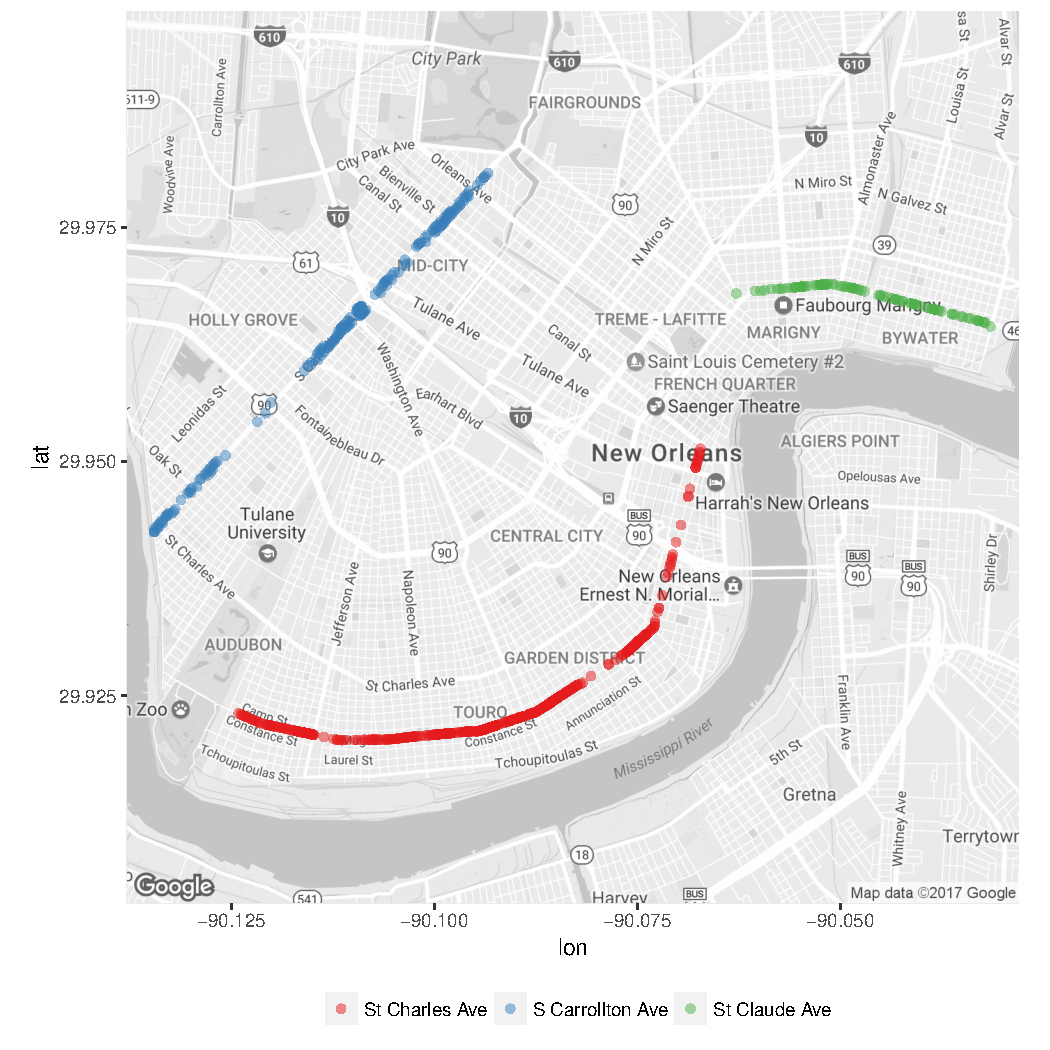
\includegraphics[scale=0.75]{img/storemap.pdf}
	\caption{Locations of all sampled stores along their respective streets}
	\label{fig:storemap}
\end{figure}



%-----------------------------------------------------------------------------
% CONCLUSTION
%-----------------------------------------------------------------------------

\section{Conclusion}\label{Conclusion}





%-----------------------------------------------------------------------------
% REFERENCES
%-----------------------------------------------------------------------------


\bibliography{Spatial_Logit.bib}{}
\bibliographystyle{unsrt}
% \bibliography{FinalProject.bib}
% \bibliography{simple}












%-----------------------------------------------------------------------------
%-----------------------------------------------------------------------------
%-----------------------------------------------------------------------------
% APPENDIX / APPENDICES
%-----------------------------------------------------------------------------
%-----------------------------------------------------------------------------
%-----------------------------------------------------------------------------

% \pagebreak

\appendix




%-----------------------------------------------------------------------------
% MAIN LEMMA 
%-----------------------------------------------------------------------------

\section{Lemma}\label{mainlemma}

\begin{lemma}\label{lem:joint}
	Define the random vectors $x$ and $\gamma$ such that the conditional distribution of $x$ given $\gamma$ and the marginal distribution of $\gamma$ are, respectively,
	%
	% 
	\begin{align*}
		(x | \gamma) &\sim \pN_n(A\gamma, \Sigma) \\
		\gamma &\sim \pN_p(m, V),
	\end{align*}
	%
	%
	where $A$ is a $n \times p$ matrix. Then the joint distribution of $(x, \gamma)^T$ is 
	%
	%
	\begin{align}
		\begin{bmatrix}
			x \\
			\gamma
		\end{bmatrix} &\sim \pN \left( \begin{bmatrix}
			Am \\
			m
		\end{bmatrix}, \begin{bmatrix}
			AVA^T + \Sigma & AV \\
			VA^T & \Sigma
		\end{bmatrix} \right). \label{eqn:lemmaresult}
	\end{align}
	%
	%
	\begin{proof}
		Equivalently, $x$ may be written as  
		%
		%
		\begin{align*}
			x = A\gamma + \eta,\; \eta &\sim \pN_n(0, \Sigma) 
		\end{align*}
		%
		%
		and then $(x, \gamma)^T$ is multivariate normal because it can be written as an affine transformation of independent multivariate normal variables,
		%
		%
		\begin{align*}
			\begin{bmatrix}
				x \\
				\gamma
			\end{bmatrix} &= \begin{bmatrix}
				A \\ 
				\mathcal{I}_p
			\end{bmatrix} \gamma + \begin{bmatrix}
				\mathcal{I}_n \\
				\mathcal{O}_{p \times n}
			\end{bmatrix} \eta. 
		\end{align*}
		%
		%
		From this, the mean and covariance matrix in (\ref{eqn:lemmaresult}) may be derived from properties of the multivatiate normal distribution.
	\end{proof}
\end{lemma} 


%-----------------------------------------------------------------------------
%-----------------------------------------------------------------------------
%-----------------------------------------------------------------------------
%-----------------------------------------------------------------------------
%-----------------------------------------------------------------------------
%-----------------------------------------------------------------------------
%-----------------------------------------------------------------------------
% END
%-----------------------------------------------------------------------------
%-----------------------------------------------------------------------------
%-----------------------------------------------------------------------------
%-----------------------------------------------------------------------------
%-----------------------------------------------------------------------------
%-----------------------------------------------------------------------------
%-----------------------------------------------------------------------------

\end{document}


